% !TEX root = ../main.tex
\chapter{Model creation} \label{ch:model}
% TITOLO DA VALUTARE
This chapter will outline the approach suggested by IBM Reserch for tackling the challange introduced in \textbf{\nameref{ch:introduction}} regarding fault detection and diagnosis (FDD). %TODO

\section{State of the art}
Nowadays, as extensively analyzed by \textcite{methods_for_diagnostic}, FDD approaches fall in either one of the following three categories: physycal model based approaches, data driven approaches and rule-based approaches. The rationales behind these approaches are detailed in \autoref{subsec:phy_models}, \autoref{subsec:data_models} and in \autoref{subsec:rule_models}.

\subsection{Physycal model approach} \label{subsec:phy_models}
These approaches require a physycal model (e.g ordinary differential equations) of the building and its components. They are highly precise in diagnosing faults given a correct model, however, deriving the models is no trivial task and requires times and expertise. On top of this, derived models are building, system and location specific and are difficult to adapt to other buildings than the one they are thought for even if they share similar structure and similar components, thus limiting the scalability of this approach.

\subsection{Data driven approach} \label{subsec:data_models}
Data driven approaches completely rely on building's sensor data. They assume that access to a large dataset of hystorical data is granted. There's little to no need for any \textit{a priori} knowledge of the processes involved. Black-box data driven approaches derive the model in the form of a input-output relationship which parameters aren't correlated with the actual physical parameter (e.g artificial neural networks, regression) while grey-box data driven approaches take advantage of simplified physical relationships between measured quantities (e.g principal component analysys) and rely on statistical methods for estimating their parameters. Even though these methods don't suffer from scalability issues they are limited to fault detection and lack in diagnosis capabilities.

\subsection{Rule-based approach} \label{subsec:rule_models}
The rule-based approach is the most common in traditional FDD applications. It uses domain knowledge and expertise in order to derive a series of simple \textit{if-then-else} rules or some kind of decision trees along with a series of thresholds and confidence intervals; during system operations data are evaluated against this rules and countermeasures are eventually taken. Even though this is the most common approach, it still needs a lot of manual effort and requires access to domain knowledge so these requirements still limit portability and scalability of applications based on this technique.

All of these approaches share common limitations that can be summarized as
\begin{itemize}
  \item they can be applied to a single, specific building
  \item they requires large manual effort and expertise
  \item deploy can take several weeks
  \item they neglect strong interactions between systems
\end{itemize}

\section{IBM Research approach}
The approach developed by IBM Research is based on a combination of the three aformentioned concepts to overcome their disadvantages. It models high level \textbf{physical processes} in the systems to derive diagnosis \textbf{rules}, it parametrize the rules using \textbf{data analytics} techniques and applies them during systmes operations. The strength of the semantic approach lies in its capability to automatically infer knowledge given a building, its sensors and their data. This lead to a semi-automated process that limit the manual effort needed as shown in \ref{fig:approach_overview}.

\begin{figure}
  \centering
  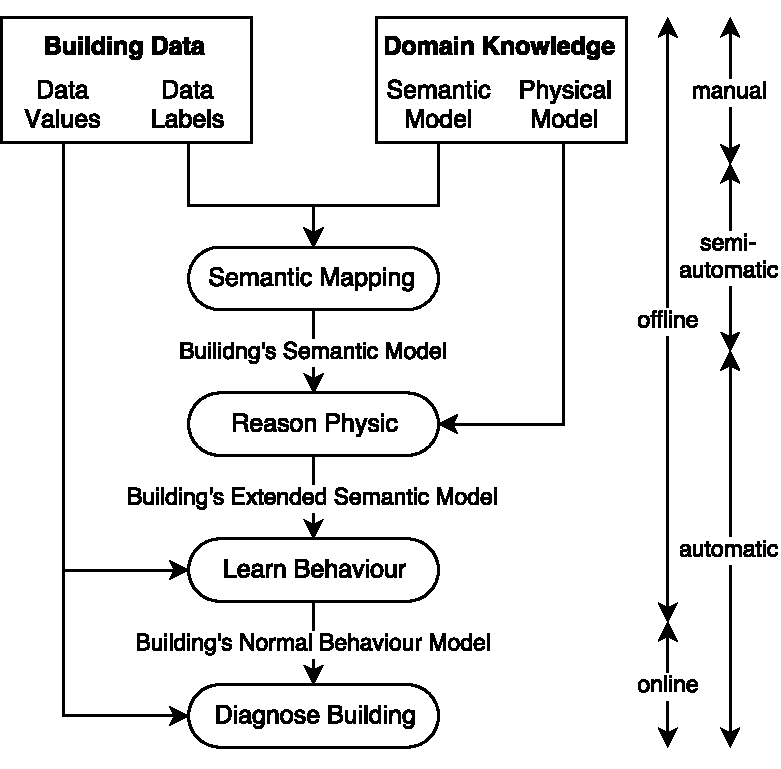
\includegraphics[width=0.7\textwidth]{approach_overview.pdf}
  \caption{IBM Reserch approach, overview}
  \label{fig:approach_overview}
\end{figure}

The proposed approach needs 3 inputs to produce the diagnosis of a given anomaly
\begin{itemize}
  \item building data: assumed available in the building's Building Management System (BMS).
  \item semantic model: specified through the use of domain ontologies Brick e SSNO.
  \item physycal model: the model of the physical dependencies between subsystems of the building. The physical processes are modelled as LTI processes described in the extended SSNO.
\end{itemize}
